\subworkpkg{1.3}

%% Tasks

%% A. Using methods based on statistical data (like, for instance, the
%% ones presented in Ref. [1]), make a first vehicle level estimation
%% of the spacecraft dry mass, power, size, reliability and
%% cost. Hint: you can use the reference spacecrafts characteristics
%% found in the framework of WP 1.2 to evaluate the accuracy of the
%% methods you have adopted, or even to develop your own estimation
%% method.

%% B. Preliminarily define the orbital parameters (a, e, i, , ) and
%% the interplanetary transfer trajectory foreseen for your mission.

%% C. Estimate the total v required by the mission and, based on
%% this, the total propellant mass needed (note: this value depends on
%% the type of engines/thrusters you use!! If this has not been
%% decided yet in detail, you may still have several open options for
%% the propellant mass at this stage…). Include in your estimation all
%% the relevant mission phases (e.g. launch, transfer, orbit
%% corrections, station keeping, interplanetary transfer, etc.). Don’t
%% forget to take into account proper margins!! Hint: you can use the
%% data referred to similar missions, found in the framework of WP
%% 1.1, as a baseline for your estimation.

%% D. Choose an adequate launcher for your mission and, consequently,
%% indicate the launch location, sketch the ascent profile, estimate
%% the maximum launch loads and the required minimum longitudinal and
%% transversal natural frequencies, and identify the payload adapters
%% available for use and their characteristics.

%% E. Based on the information obtained from the previous Tasks,
%% generate a detailed mission profile and a rough timeline for the
%% mission.

%% Deliverables

%% D1.3.1. Vehicle-level estimation of the spacecraft dry mass,
%% propellant mass, power, size, reliability and cost.

\deliverable{1.3.1 Vehicle-Level Estimation}

In this section some vehicle-level estimations of the spacecraft are
given in order to identify the most important design parameters.

\subsection{Dry mass}
\label{sec:drymass}

For the vehicle dry mass estimation, some reference spacecrafts were
used. The dry mass of the reference spacecrafts was plotted against
the payload in the figure below.

\begin{figure}[h]
  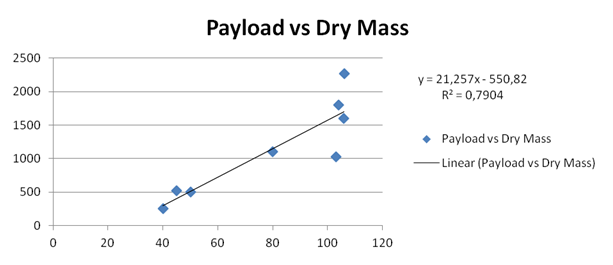
\includegraphics[width=\textwidth]{Payload-vs-DryMass}
  \caption{Payload vs. Dry Mass}
\end{figure}

The data shown in the figure above was used to estimate the dry mass
of the satelite to be designed, which was found to be \SI{1100}{kg}.

\subsection{Power}
\label{sec:power}

From the reference data it can be seen that the typical used power is
between \SI{400}{W} and \SI{636}{W} with a payload of
\SI{105}{kg}. With the used payload in mind, the estimated range is
between \SI{305}{W} and \SI{485}{W}.

\subsection{Reliability}

The required mission reliability has to be higher than 0.9. From this
requirement the failure rate $\lambda$ can be determined.

\begin{equation}
  \lambda = \frac{\ln R}{t}
\end{equation}

This leads to a failure rate of 0.01317 failures per year for a
lifespan of 6.2 years.

\subsection{Initial mass}
\label{sec:initialmass}

To calculate the total mass of the spacecraft, Tsiolkovsky's rocket
equation is used

\begin{equation}
  \Delta V = V_e \ln \frac{M_0}{M_1}
\end{equation}

\begin{equation}
  M_0 = M_1 \exp \frac{\Delta V}{V_e}
\end{equation}

The $\Delta V$ has been calculated in a previous part and is found to
be \SI{2.625}{km/s}. The exhaust velocity is determined by the
specific impulse multiplied with the gravitational acceleration of
Earth. An estimated $I_{\mathrm{sp}}$ of \SI{318}{s} is used, leading to an
exhaust velocity of \SI{3117}{m/s}. Finally, an initial mass of
\SI{2550}{kg} is found. Since the calculation assumes ideal conditions
an additional margin of \SI{20}{\%} is used, leading to an estimation
of \SI{3000}{kg} for the initial mass of the spacecraft.

\subsection{Sizing}

In order to estimate the size of the spacecraft, an average mass
density of \SI{79}{kg/m^3} is used as this value was indicated in
\textit{Space Mission Engineering: The New SMAD}
\cite{Wertz2011SpaceMissionEng}. Using the following relation,

\begin{equation}
  V = \frac{M}{\rho}
\end{equation}
an estimated size of \SI{38}{m^3} is determined.

\subsection{Cost}

The cost of the spacecraft can be estimated upon the dry mass using
the following relationship\cite{AE1201CourseReader},

\begin{equation}
  C_{\mathrm{S/C}} = 0.3531 (M_{\mathrm{dry}})^{0.839}
\end{equation}
resulting in a spacecft cost of 125.8 million dollars.

%% D1.3.2. Complete mission profile (including a description of the
%% launcher requirements and characteristics) and preliminary mission
%% timeline up to EOL (End Of Life).

\pagebreak
\deliverable{1.3.2 Complete Mission Profile}

\begin{longtable}{lp{.8\textwidth}}
  \caption{Mission Timeline.} \\

  Duration & Launch \\ \cmidrule{2-2}

  $\le$ \SI{1}{h}

  & Launch of the spacecraft by Falcon9 into GTO \\ \midrule

  Duration & From separation to Earth gravity assist \\ \cmidrule{2-2}

  2 years

  & This is an average time taken for Juno and Galileo spacecraft to
  go from separation to Earth gravity assist. \\ \midrule

  Duration & From Earth gravity assist to Jupiter orbit \\ \cmidrule{2-2}

  2.7 years

  & This transfer time was calculated as if Hohmann interplanetary
  transfer (elliptical orbit) was used, and the calculated value was
  double-checked with the actual transfer time for Juno and JEO
  mission; both approximately 3 years, very close to the calculated
  result.

  \begin{equation}
    T_{\mathrm{transfer}}
    =\pi\sqrt{\frac {a^3}{\mu_{\mathrm{sun}}}}
    =\pi\sqrt{\frac{(\SI{3.1}{AU})^3}{\SI{1.327d11}{km^3/s^2}}}
  \end{equation} \\ \midrule

  Duration & Orbiting Jupiter until the departure for Europa Orbit
  Insertion \\ \cmidrule{2-2}

  4 days

  & One full orbit around Jupiter was assumed as a preparation time
  for the departure towards Europa orbit.  This is simply calculated
  as if the spacecraft is circulating in Europa's orbit, which has
  the radius of 671000km from Jupiter.

  \[ \begin{aligned}
    T_{\mathrm{orbit}}
    &= 2\pi\sqrt{\frac{a^3}{\mu_{\mathrm{jupiter}}}} \\
    &= 2\pi\sqrt{\frac
      {(\SI{671000}{km})^3}
      {\SI{126686534}{km^3/s^2}}} \\
    &= 3.6\,\mathrm{days}
  \end{aligned} \] \\ \midrule

  Duration & Europa orbit insertion \\ \cmidrule{2-2}

  2 days

  & The target orbit around Europa has a much smaller radius of
  \SI{1760}{km} compared to the radius of Europa's orbit around
  Jupiter (\SI{671000}{km}).  Under the assumption that the Europa
  orbit insertion is done from one point of the Jovian orbit to the
  right opposite side of the orbit, the transfer time can be
  approximated as half the orbit period of Europa around Jupiter which
  would be around 2 days. \\
\end{longtable}

%% D1.3.3. Graphical sketch of the spacecraft trajectory during all
%% the phases of the mission, including launch, ascent, separation,
%% parking orbit(s), interplanetary transfer and final orbit.

\deliverable{1.3.3 Spacecraft Trajectory}

The spacecraft trajectory during all mission phases has been sketched
in two parts. The first part shows a sample ascent profile of the
Falcon9 rocket, whereas the second sketch includes all transfer orbits
that will be used to reach Europa.

\begin{figure}[H]
  \center
  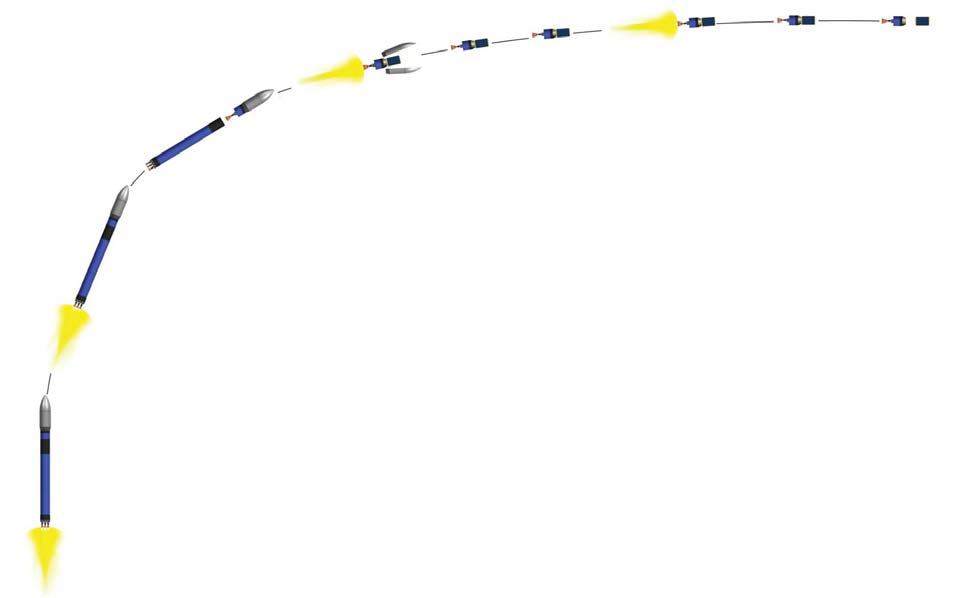
\includegraphics[width=.8\textwidth]{Launch-Profile}
  \caption{Sample Launch Profile: Falcon9 \cite{LVCFalcon9}}
\end{figure}

\begin{figure}[H]
  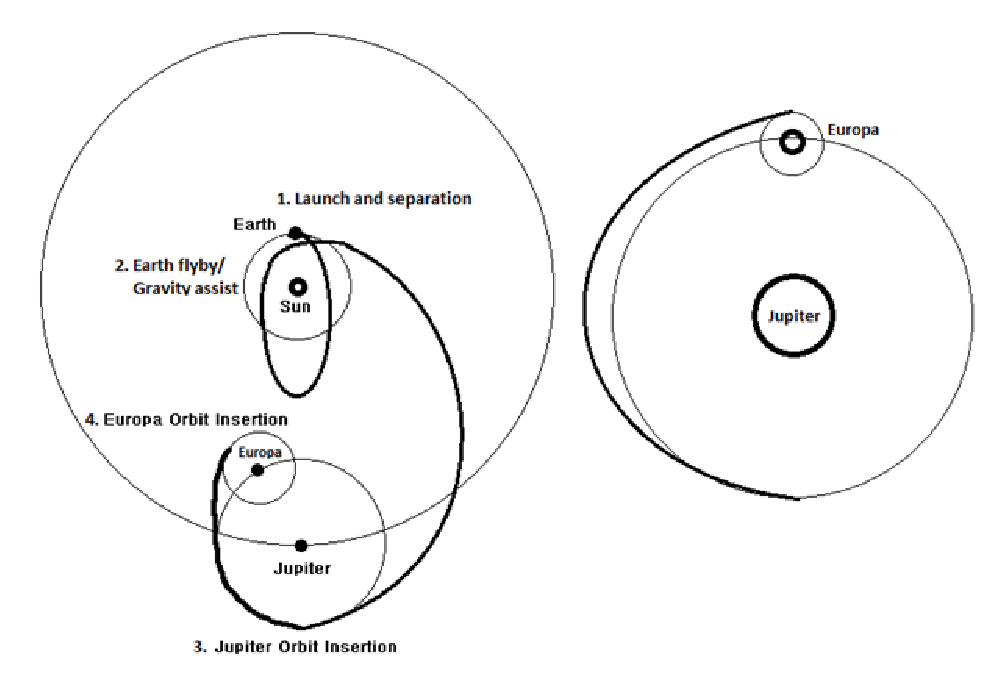
\includegraphics[width=\textwidth]{Mission-Profile}
  \caption{Complete Mission Profile}
\end{figure}

%% D1.3.4. Table showing the orbital parameters characterizing the
%% spacecraft final orbit.

\deliverable{1.3.4 Orbital Parameters}

The orbital parameters which characterize the spacecrafts final orbit
can be obtained from the table below.

\begin{longtable}{ll}
  \caption{Orbital Parameters \cite{JupiterFactSheet}} \\

  Earth-Sun distance & \SI{1}{AU} \\

  Jupiter-Sun distance & \SI{5.2}{AU} \\

  $\mathrm{\mu_{Sun}}$ & \SI{1.327d11}{km^3/s^2} \\

  $\mathrm{\mu_{Jupiter}}$ & \SI{1.267d8}{km^3/s^2} \\

  Europa-Jupiter distance & \SI{671000}{km} \\

  Europa target orbit altitude & \SI{200}{km} \\

  Europa target orbit radius & \SI{1760}{km} \\

  Semimajor axis of transfer from Earth to Jupiter

  & \SI{3.1}{AU} \\

  Eccentricity of transfer & 0.677 \\

  Inclination of transfer relative to the ecliptic plane & \ang{1;3;1}
  \\
\end{longtable}


%% D1.3.5. Estimated total v required by the mission, including a
%% table showing its breakdown into all the contributions related to
%% different mission phases and operations.

\deliverable{1.3.5 Estimated delta-V Budget}

The most traditional interplanetary transfer, the direct Hohmann
transfer orbit can be considered for this mission, since this method
has high efficiency, rapid transfer, and low radiation
exposure.\cite{Wertz2011SpaceMissionEng}

\begin{figure}[H]
  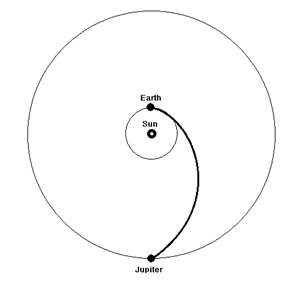
\includegraphics[width=\textwidth]{Hohmann-Orbit}
  \caption{Interplanetary Hohmann-Transfer-Orbit to Jupiter}
\end{figure}

To simplify the calculations it is assumed that both, Earth and
Jupiter, orbit the Sun in a perfectly circular orbit.  The required
orbital parameters are taken from the previous section.  Using
Hohmann-Transfer-Orbits we obtain

\begin{align*}
  \Delta V_{total} = {} &
  \Delta V_{\mathrm{perigee}}
  + \Delta V_{\mathrm{apogee}} \\
  = {} & \sqrt{\frac{\mu_{\mathrm{sun}}}{r_{\mathrm{earth}}}}
  - \sqrt{\mu_{\mathrm{sun}} \left(\frac{2}{r_{\mathrm{earth}}}
    - \frac{1}{a_{\mathrm{transfer}}}\right)} \\
  + & \sqrt{\frac{\mu_{\mathrm{sun}}}{r_{\mathrm{jupiter}}}}
  - \sqrt{\mu_{\mathrm{sun}}\left(\frac{2}{r_{\mathrm{jupiter}}}
    - \frac{1}{a_{\mathrm{transfer}}}\right)} \\
  \approx {} & \SI{8.78}{km/s} + \SI{5.63}{km/s} = \SI{14.41}{km/s} \\
\end{align*}

Given that $\Delta V_\mathrm{perigee}$ (\SI{8.78}{km/s}) is achieved
by the launcher rocket, the total $\Delta V$ that the spacecraft has
to carry itself is \SI{5.63}{km/s} which is still rather high compared
to similar existing missions, such as Juno or JUICE (See WP1.1 for
details).  Thus, it can be concluded that the Hohmann interplanetary
transfer orbit in this case does not give the most practical/optimum
trajectory for the mission.  One of the solutions to reduce the high
$\Delta V$ is to use gravity assist, which basically makes use of the
gravity of other planets during the flyby to induce a “slingshot”
effect.  Two of the existing reference missions to Jupiter use such
method to arrive at the planet Jupiter’s orbit; Galileo and Juno.  As
discussed in WP 1.1, Galileo has gravity assist of Venus-Earth-Earth,
and Juno has gravity assist of Earth.  Compared to Galileo, the Juno
spacecraft took almost 14 month less time to get to
Jupiter.\cite{SolarSystemNasa} Considering the fact that the Juno
mission shares many similar aspects with our own mission to Europa,
the mission profile of Juno can be considered as a model for our
mission.  Using one gravity assist of Earth, the orbit transfer
trajectory can be designed as shown in the figure below.

\begin{figure}[H]
  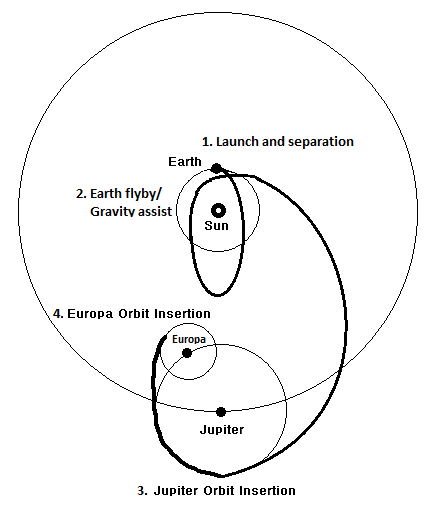
\includegraphics[width=\textwidth]{Transfer-Orbits}
  \caption{Orbit transfer trajectory using one Earth gravity assist}
\end{figure}

It should be noted that the spacecraft may temporarily orbit around
the Jupiter several times in order to achieve Europa Orbit insertion
in a favorable time and position, preferably with the minimum
$\Delta V$ and thus, the least fuel consumption. Using the data from
the Juno mission, the total $\Delta V$ budget can be estimated
\cite{DMullerNet} ($\Delta V$ for the Europa orbit insertion was taken
from the other source since the Juno mission is mainly orbiting the
planet Jupiter rather than its moon Europa). \cite{TrajectoryDesign}

\begin{table}[H]
  \caption{$\Delta V$ Breakdown}
  \begin{tabular}{ll}
  Maneuver & $\Delta V$ \si{km/s} \\

  Deep space maneuver after launch until arrival at Jupiter & 733 \\

  Jupiter orbit insertion and period adjustment & 1072 \\

  Europa orbit insertion & 720 \\

  Possible orbit correction maneuver ($\Delta V$ margin) & 100 \\

  Total $\Delta V$ for spacecraft & 2625 \\
  \end{tabular}
\end{table}

Therefore, assuming the specific impulse of \SI{318}{s} (bipropellant
system with nitrogen tetroxide/monomethylhydrazine propellants which
is the propulsion system used for Galileo --- additional remark: a
bipropellant system is also used for the Juno and the JUICE
mission)\cite{Ampac}, the required propellant mass for the spacecraft
can be calculated from the rocket equation:

\begin{equation}
  \Delta V = V_e \ln \frac{M_0}{M_1}
  = I_{\mathrm{sp}} \, g_0 \ln \frac{M_0}{M_1}
\end{equation}
\begin{equation}
  M_{\mathrm{propellant}}
  = M_1 \left( \exp \frac{\Delta V}{I_{\mathrm{sp}} \, g_0} - 1 \right)
    \approx 1.223 M_1
\end{equation}
